\documentclass[french,a4paper,11pt]{report}
\usepackage[T1]{fontenc}
\usepackage{fourier}
\usepackage[utf8]{inputenc}
\usepackage[french]{babel}
\usepackage{hyperref}
\usepackage{biblatex}
\usepackage{xcolor}
\usepackage[scale=0.8]{geometry}

\usepackage{listings}
\lstset{basicstyle=\ttfamily,
  showstringspaces=false,
  basicstyle=\footnotesize\ttfamily,
  keywordstyle=\bfseries\color{green!40!black},
  commentstyle=\color{purple!40!black},
  identifierstyle=\color{blue},
  stringstyle=\color{red},
  breaklines=true,
  frame=l, % single, L, lines
  framerule=2pt
}

\usepackage{graphicx}
\graphicspath{ {images/} }

\usepackage{lastpage}
\usepackage{fancyhdr}


\cfoot{\thepage\ of \pageref{LastPage}}

% \fancyhead{} % clear all header fields
% \fancyhead[C]{\scriptsize Notre beau titre}
% \fancyfoot{}
% \fancyfoot[C]{\thepage/\pageref{LastPage}} % clear all footer fields
% %\fancyfoot[LE,RO]{}
% %\fancyfoot[RE,LO]{\scriptsize Webs'INT - Télécom SudParis}
% \fancyfoot[CO,RE]{}
% %\renewcommand{\headrulewidth}{0pt}
% %\renewcommand{\footrulewidth}{0pt}

\title{Environnements de TP pour MOOC}
\author{François Monniot \& Alexis Mousset}

% PDF metadata
\hypersetup{pdfinfo={
  Author={François Monniot, Alexis Mousset},
  Title={Adding PDF metadata in LaTeX},
  Keywords={MOOC;Docker;TSP}
}}

\addbibresource{report.bib}

\begin{document}

\maketitle
\tableofcontents

\begin{abstract}

\end{abstract}
\pagestyle{fancy}
\chapter{Introduction}
\pagestyle{fancy}
\section{MOOC}

\subsection{Contexte des MOOC à TSP et en général}

\subsection{Contexte des besoins de TP}

Télécom SudParis a lancé son premier MOOC en décembre 2013.

\section{Solution apportée}

\subsection{Expression précise du besoin}

Le besoin exprimé dans le cadre de notre projet de fin d'études est la gestion d'environnements de travaux pratiques pour des MOOC, notamment les MOOC mis en place à Télécom SudParis. Un environnement de TP est déjà en place pour le MOOC de bases de données, basé sur Vagrant.

Ces environnements doivent pourvoir êtres utilisés sur les postes des apprenants, et éventuellement aussi sur un serveur. Cela impose plusieurs contraintes :
\begin{itemize}
  \item Compatibilité logicielle : utilisable sur la grande majorité de systèmes d'exploitation, même dans des version anciennes
  \item Compatibilité matérielle : utilisable sur du matériel ancien et peu performant
\end{itemize}

Ces environnements doivent aussi être faciles à créer et ne nécessitent que peu de compétences
particulières.

\subsection{Qu'est-ce que Docker ?}

Docker\cite{website:whatis-docker} a été lancé en tant que projet open-source en mars 2013.
C'est un programme permettant de gérer le déploiement d'un type de virtualisation particulier : les conteneurs.
  
\subsection{Adéquation de la solution}

Utilisation de boot2docker, qui installe VirtualBox, MSYS-git

tiny core linux : 27MB de RAM dans  boot2docker

Par rapport à Vagrant :
\begin{itemize}
  \item Mêmes besoins matériels : support de la virtualisation, 2 Go de RAM pour un usage confortable.
  \item Le principal obstacle au niveau compatibilité est la nécessité d'un OS 64 bit.
  \item Au niveau professeur, utilisation de scripts pour la mise en place. Facilité de migration vers Docker.
  \item Au niveau apprenant, installation légèrement plus simple (boot2docker), et mise à jour facilitée en utilisant les mises à jour incrémentales des images docker.
  \item Plus orienté production si utilisation sur un serveur.
\end{itemize}

\subsubsection{Compatibilité logicielle}

Docker nécessite en général un noyau linux supérieur à 3.8 (sorti en février 2013) à cause d'un bug LXC\cite{website:bug-lxc} présent dans les versions antérieures, ainsi qu'un noyau 64 bit.

Distribution pleinement compatibles :
\begin{itemize}
  \item Ubuntu à partir de la 13.04, notamment Ubuntu 14.04 LTS.
  \item Debian à partir de la version 8
  \item RHEL/CentOS à partir de la version 7
  \item RHEL à partir de la version 6.5 avec un noyau supérieur à 2.6.32-431, qui contient le patch nécessaire à Docker. Docker doit être installé de puis les dépôts EPEL.
\end{itemize}

Distribution compatibles après adaptations :
\begin{itemize}
  \item Ubuntu 12.04 LTS (kernel backporté)
  \item Debian 7 (kernel backporté)
  \item RHEL 6 à partir de la version 6.5 avec un noyau supérieur à 2.6.32-431, qui contient le patch nécessaire à Docker (docker doit être installé de puis les dépôts EPEL)
\end{itemize}

Un résumé de la compatibilité est présenté dans le tableau \ref{tab-linux}.

\begin{figure}[h!]
\begin{center}
  \begin{tabular}{| c | c | c | }
     \hline
     Distribution & Support natif & Support après adaptation \\ \hline
     Debian & 8 (jessie) & 7 (wheezy) \\ \hline
     Ubuntu & 13.04, 13.10, 14.04 LTS, 14.10 & 12.04 LTS \\ \hline
     RHEL/CentOS & 7 & 6.5, 6.6 \\
     \hline
   \end{tabular}
      \end{center}
  \caption{Compatibilité logicielle de Docker sous Linux}
  \label{tab-linux}
\end{figure}

En cas de problème de version kernel, il est possible d'utiliser la même méthode que boot2docker et installer une VM utilisant un noyau récent (par exemple un CoreOS).

Sous Windows et MacOS, la compatibilité est celle de VirtualBox (à partir de Windows XP), avec la contrainte supplémentaire d'un OS 64 bit, ce qui en pratique ne retient que les systèmes postérieurs à Windows Vista (surtout à partir de Windows 7) et Mac OS X 10.5. 

\subsubsection{Compatibilité matérielle}

Comme toute solution basée sur la virtualisation, l'utilisation nécessite un processeur avec support de la virtualisation matérielle. Boot2docker demande aussi un minimum de 2Go de RAM.

Docker nécessitant un hôte 64bit, l'hôte de boot2docker doit aussi être en 64bit. En général la limitation est logicielle, les processeurs supportant la virtualisation étant en général en 64bit. Les processeurs 64bit recouvrent les processeurs :

\begin{itemize}
  \item AMD à partir de 2003 avec les Opteron et Athlon 64
  \item Intel à partir de 2004 avec certains Pentium 4 et Xeon, sauf Atom et Celeron jusqu'à 2008.
\end{itemize}

Le tableau \ref{compat} résume la compatibilité des environnements basés sur docker.

   \begin{figure}[h!]
\begin{center}
   \begin{tabular}{| c | c |}
     \hline
     Caractéristique & Minimum \\ \hline
     RAM & 2Go \\ \hline
     Disque & 1Go disponible \\ \hline
     Mac OS X & 10.5 en \textbf{64 bit} \\ \hline
     Linux & 3.8 et 2.6.32-431 RHEL en \textbf{64 bit} \\ \hline
     Windows & (Vista), 7, 8, 8.1 en \textbf{64 bit} \\
     \hline
   \end{tabular}
   \end{center}
   \caption{Compatibilité matérielle et logicielle}
   \label{compat}
  
\end{figure}

\chapter{Implémentation}

\section{Partie agent}


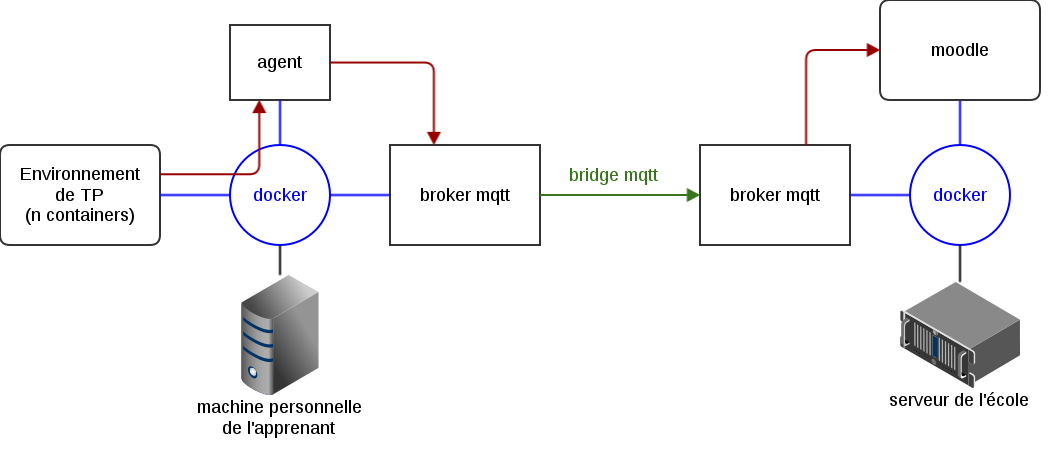
\includegraphics[scale=0.45]{docker}

Parite agent en python

bug streaming logs

scéma de nommage

%erreur mqtt : https://bugs.eclipse.org/bugs/show_bug.cgi?format=multiple&id=446062

faire un filtre dans l'agent


\section{Partie moodle}

\subsection{}

\subsection{}

\pagestyle{fancy}

\chapter{Utilisation}

\pagestyle{fancy}

\section{Cas d'utilisation : Le MOOC bases de données}

\subsection{Infrastructure}

Construction des images

docker hub

moodle

\subsection{Côté professeur}

L'objectif côté professeur est de faciliter la mise en place d'environnements de TP par des non spécialistes de docker (éventuellement assistés en cas de problèmes).
La configuration des machines de TP s'effectue sur un dépôt git contenant les scripts de création des environnements, ainsi que les contenus qui y seront ajoutés. Les images sont ensuite générées et déposées.
Le format de configuration est le Dockerfile, qui est constitué d'une suite de commandes lancées et de copies de fichiers. Il est très simple, si on sait configurer un système, de le consigner dans un Dockerfile.

La mise en place des TP de ce MOOC nécessite deux conteneurs : un pour la base de données et un pour le serveur et les applications web, ainsi que du conteneur permettant le suivi.

\begin{lstlisting}[language=Bash,caption={Dockerfile de base}]
RUN apt-get update && apt-get install my_software
COPY configuration_file /etc/my_software/
EXPOSE 80
# The command that should be executed
CMD ["/usr/bin/my_software"]
\end{lstlisting}

Le conteneur de base de données est basé sur l'image postgreSQL officielle (elle même basée
sur Debian). La configuration et le peuplement des bases de données sont effectuées à partir d'un script shell appelé lors de la création du conteneur. Ce script appelle les scripts de peuplement sql, et permet de créer les utilisateurs nécessaires.

L'image web est basée sur debian, sur laquelle est installée apache et phppgadmin. De plus des fichiers suppmémentaire sont ajoutés dans un autre virtualhost, qui contient donc les fichiers applicatifs liés au TP.

Une fois le container lancé, l'insterface web est accessible en local sur la machine.

\subsection{Côté apprenant}

L'apprenant doit d'abord installer boot2docker, qui se charge d'installer git et virtualbox s'ils ne sont pas présents. Le téléchargement est de 122 Mo. L'installeur ajoute un raccourci dans les menus permettant d'accéder à un shell sur le VM boot2docker, sans avoir à passer par virtualbox. Ensuite l'apprenant doit exécuter des commandes permettant de récupérer les images correspondant à son TP, puis à les lancer. Il peut ensuite accéder à son environnement de TP.

% todo : doc apprenant

overview ?


\printbibliography

\end{document}
